\documentclass{packages/sysuthesis} % 默认使用电子版（不填充空白页）。如果需要双面打印版，请注释掉本行并启用下一行
\usepackage{packages/sysucode}  % 在论文中使用代码
\usepackage{xurl}
\usepackage[most]{tcolorbox} % 支持附录中的问答彩色框
\pgfplotsset{compat=1.18,compat/show suggested version=false} % 固定兼容版本并关闭提示信息
\setlength{\headheight}{13pt} % 消除 fancyhdr 的 headheight 告警
\covertitlefirst{编译原理}
\covertitlesecond{实验课第五次作业}
\ctitle{编译原理——实验第五次作业: 逆向工程工具 ROSE}
\cauthor{林宏宇}
\studentid{23320093}
\cschool{计算机学院}
\cmajor{计算机科学与技术}
\emajor{Computer Science and Technology}
\cmentor{李文军}
     % 论文相关信息
% 中文
\cabstract{
本实验基于 Oberon-0 语言定义 \cite{lab05}，设计并实现了一个面向 Oberon-0 语言的逆向工程工具 ROSE（Reverse Oberon Software Engineering）。实验分为四个子实验：实验一通过编写正确的 Oberon-0 源程序及其变异程序，深入理解 Oberon-0 语言的词法、语法和语义定义，讨论了保留字与关键字的区别以及文法的二义性问题；实验二利用词法分析程序自动生成工具 JFlex，编写 Oberon-0 语言的词法规则正则定义式，自动生成词法分析程序并对三种 lex 族工具进行比较；实验三使用语法分析程序自动生成工具 JavaCUP，编写 Oberon-0 语言的语法规则和语义动作，自动生成支持调用图绘制的语法分析与语法制导翻译程序；实验四手工设计 Oberon-0 语言的翻译模式，采用递归下降预测分析技术编写语法分析程序，实现流程图自动生成，并对自顶向下与自底向上两种分析策略进行了深入的比较分析。本实验通过 ROSE 工具的完整设计与实现，帮助学生深入理解和牢固掌握编译技术中的词法分析、语法分析、语法制导翻译以及自动生成工具等重要环节。
% TODO：等待补充结果摘要
}

\ckeywords{编译原理；Oberon-0；逆向工程；词法分析；语法分析；JFlex；JavaCUP；递归下降；ROSE}     % 摘要内容
\definecolor{codebg}{RGB}{248,249,250}
\definecolor{codeframe}{RGB}{220,223,228}
\definecolor{codekw}{RGB}{25,85,145}
\definecolor{codecm}{RGB}{90,125,90}
\definecolor{codestr}{RGB}{136,44,136}
\lstdefinestyle{cleanjava}{
  language=Java,
  basicstyle=\ttfamily\small,
  keywordstyle=\bfseries\color{codekw},
  commentstyle=\itshape\color{codecm},
  stringstyle=\color{codestr},
  backgroundcolor=\color{codebg},
  frame=single,
  rulecolor=\color{codeframe},
  framesep=6pt,
  numbers=left,
  numberstyle=\scriptsize\color{gray},
  numbersep=8pt,
  breaklines=true,
  breakatwhitespace=false,
  showstringspaces=false,
  keepspaces=true,
  tabsize=4,
  columns=fullflexible
}
 % 共享的代码样式定义（必须在导言区）

\begin{document}

\frontmatter
\pagenumbering{Roman}
\makeUndergraduateCover

\makecabstract
\newpage
\maketableofcontents
\mainmatter

\chapter*{实验目的}

本实验旨在设计并实现一个面向 Oberon-0 语言的逆向工程工具 ROSE（Reverse Oberon Software Engineering），通过完整的词法分析、语法分析和语法制导翻译过程，深入理解和掌握编译原理中的核心技术。实验分为四个子实验：

\begin{itemize}
  \item \textbf{实验一：熟悉 Oberon-0 语言定义}。通过编写正确的 Oberon-0 源程序及其变异程序，深入理解 Oberon-0 语言的词法、语法和语义定义，讨论保留字与关键字的区别以及文法的二义性问题。
  \item \textbf{实验二：利用 JFlex 自动生成词法分析程序}。编写 JFlex 输入源文件 \texttt{oberon.flex}，自动生成词法分析程序，比较三种 lex 族工具。
  \item \textbf{实验三：利用 JavaCUP 自动生成语法分析程序}。编写 JavaCUP 输入源文件 \texttt{oberon.cup}，实现调用图自动生成，比较 yacc 族工具。
  \item \textbf{实验四：手工编写递归下降预测分析程序}。设计翻译模式，编写递归下降分析程序，实现流程图自动生成，比较自顶向下与自底向上策略。
\end{itemize}


\chapter*{项目组织}

本实验项目的 ROSE 软装置提供了预定义的调用图 API（\texttt{callgraph} 包）和流程图 API（\texttt{flowchart} 包），基于开源项目 JGraph。软装置不包含异常类的完整实现（参见 Notation.md），需学生自行完善。

\section*{目录组织}

\begin{itemize}
  \item \textbf{ex1/}：实验一结果目录。
    \begin{itemize}
    \item \texttt{testcases/BankSystem.obr}：正确的 Oberon-0 源程序，覆盖全部语法构造。
    \item \texttt{testcases/BankSystem.001--022}：22 个变异程序（14 个直接构造 + 8 个 derived 派生），首行注释标注期望错误类型和变异来源。
    \end{itemize}
  \item \textbf{ex2/}：实验二结果目录（JFlex 词法分析）。
    \begin{itemize}
    \item \texttt{src/oberon.flex}：JFlex 输入源文件，自动生成 \texttt{OberonScanner.java}（NFA 263 → DFA 105）。
    \item \texttt{src/exceptions/}：自行完善的 14 个异常类三层继承体系（软装置标记为 [PENDING]）。
    \item \texttt{bin/}、\texttt{doc/}、\texttt{jflex/}：字节码、javadoc 文档、JFlex 1.8.2 工具包。
    \item \texttt{gen.bat}、\texttt{build.bat}、\texttt{run.bat}、\texttt{test.bat}：生成、构建、运行和测试脚本。
    \end{itemize}
  \item \textbf{ex3/}：实验三结果目录（语法分析 + 调用图）。
    \begin{itemize}
    \item \texttt{src/oberon.cup}：JavaCUP 输入源文件，经 JavaCUP 0.11b 生成 \texttt{Parser.java} + \texttt{Sym.java}（190 状态，0 冲突）。
    \item \texttt{src/ScannerAdapter.java}：适配 OberonScanner Token 到 CUP Symbol 接口。
    \item \texttt{src/Scope.java}：链式作用域，支持嵌套过程的正向名称查找。
    \item \texttt{bin/}、\texttt{doc/}、\texttt{javacup/}：字节码、javadoc 文档、JavaCUP 0.11b 工具包。
    \end{itemize}
  \item \textbf{ex4/}：实验四结果目录（递归下降 + 流程图）。
    \begin{itemize}
    \item \texttt{src/OberonParser.java}：手工编写的递归下降预测分析器，含翻译模式设计和 flowchart API 集成。
    \item \texttt{src/OberonScanner.java}、\texttt{src/Token.java}：复用实验二的词法分析器。
    \item \texttt{bin/}、\texttt{doc/}：字节码、javadoc 文档。
    \item \texttt{build.bat}、\texttt{run.bat}、\texttt{test.bat}：构建、运行和测试脚本。
    \end{itemize}
\end{itemize}
     % 总体实验目的 + 项目组织
\newclearpage
\chapter{实验一：熟悉 Oberon-0 语言定义}

\section*{实验目的}

本实验（实验一）旨在深入理解 Oberon-0 语言的定义，为后续词法分析、语法分析和语法制导翻译实验奠定基础。具体目标包括：

\begin{itemize}
    \item 阅读 Oberon-0 语言的 BNF 定义和语义描述，掌握该语言的完整语法规则。
    \item 编写一个词法、语法和语义均正确的 Oberon-0 源程序，覆盖所有语法构造。
    \item 基于变异测试思想，针对每一种可能的词法、语法和语义错误构造变异程序。
    \item 讨论 Oberon-0 语言的特点（保留字与关键字的区别、表达式语法的独特性）。
    \item 分析 Oberon-0 文法的二义性，理解其与其他高级语言在语法设计上的差异。
\end{itemize}

\section*{实验目录与项目组织}

实验一的项目文件均存放于 \texttt{ex1/} 子目录下，各文件说明如下：

\begin{itemize}
    \item \texttt{readme.txt}：自述文件，包含姓名、学号、完成日期及补充说明。
    \item \texttt{testcases/BankSystem.obr}：词法、语法、语义均正确的 Oberon-0 源程序，覆盖了语言的全部语法构造。
    \item \texttt{testcases/BankSystem.001--022}：22 个变异程序（14 个直接构造 + 8 个 derived 派生），分别包含一种词法、语法或语义错误，首行注释标明期望异常类型和变异来源。文件扩展名以数字序号区分。
\end{itemize}

\section{正确的 Oberon-0 源程序}

根据 Oberon-0 语言的 BNF 定义，编写了一个模拟银行账户管理系统的 Oberon-0 源程序 \texttt{BankSystem.obr}，覆盖了 Oberon-0 语言的所有主要语法构造：

\begin{itemize}
    \item \textbf{模块声明}：MODULE BankSystem ... END BankSystem.
    \item \textbf{常量声明}：CONST MaxAccounts = 50; MinBalance = 100;
    \item \textbf{类型声明}：TYPE AccountRec = RECORD ... END; TYPE AccountArray = ARRAY 50 OF AccountRec;
    \item \textbf{变量声明}：VAR accounts, count, i, choice, amount, accId: INTEGER; VAR running, found: BOOLEAN;
    \item \textbf{过程声明}（5 个）：InitAccounts、FindAccount（含 VAR 参数）、Deposit、Withdraw、CreateAccount
    \item \textbf{IF 语句}：含 IF-THEN-ELSE、IF-THEN-ELSIF-THEN-ELSE-END 等完整形式
    \item \textbf{WHILE 循环语句}
    \item \textbf{赋值语句}：含数组下标选择（\texttt{accounts[k].id := 0}）和记录域选择（\texttt{accounts[k].balance := 0}）
    \item \textbf{过程调用}：含实际参数传递
    \item \textbf{预定义过程调用}：Read、Write、WriteLn
    \item \textbf{布尔变量与逻辑运算}：\texttt{~found}、\texttt{(j < count) \& ~found}
\end{itemize}

程序具有实际意义：实现银行账户的创建、存款、取款等基本操作，展示了 Oberon-0 作为教学语言的核心抽象能力。

\section{变异程序}

\begin{table}[htbp]
    \centering
    \begin{tabular}{|c|c|c|c|}
    \hline
    \textbf{变异程序} & \textbf{类别} & \textbf{错误描述} & \textbf{检测结果} \\
    \hline
    BankSystem.001 & 词法 & 非法符号 \$ & IllegalSymbolException $\checkmark$ \\
    BankSystem.002 & 词法 & 标识符超 24 字符 & IllegalIdentifierLengthException $\checkmark$ \\
    BankSystem.003 & 词法 & 非法八进制 08 & IllegalOctalException $\checkmark$ \\
    BankSystem.004 & 词法 & 25id 无空白分隔 & IllegalIntegerException $\checkmark$ \\
    BankSystem.005 & 词法 & 注释未闭合 & MismatchedCommentException $\checkmark$ \\
    BankSystem.014 & 词法 & 整数超12位 & IllegalIntegerRangeException $\checkmark$ \\
    BankSystem.006 & 语法 & 缺左括号 & MissingLeftParenthesisException $\checkmark$ \\
    BankSystem.007 & 语法 & 缺右括号 & MissingRightParenthesisException $\checkmark$ \\
    BankSystem.008 & 语法 & 两表达式间缺运算符 & MissingOperatorException $\checkmark$ \\
    BankSystem.009 & 语法 & 二元运算缺右操作数 & MissingOperandException $\checkmark$ \\
    BankSystem.010 & 语法 & 缺 END & SyntacticException $\checkmark$ \\
    BankSystem.011 & 语义 & INTEGER \& BOOLEAN & TypeMismatchedException $\checkmark$ \\
    BankSystem.012 & 语义 & 参数数目不匹配 & ParameterMismatchedException $\checkmark$ \\
    BankSystem.013 & 语义 & 模块名不匹配 & SemanticException $\checkmark$ \\
    BankSystem.015 & 词法 & 非法符号 @ & IllegalSymbolException $\checkmark$ \\
    BankSystem.022 & 词法 & 非法八进制 09 & IllegalOctalException $\checkmark$ \\
    BankSystem.021 & 词法 & 注释未闭合 & MismatchedCommentException $\checkmark$ \\
    BankSystem.017 & 语法 & 缺左括号 & MissingLeftParenthesisException $\checkmark$ \\
    BankSystem.016 & 语法 & 缺右括号 & MissingRightParenthesisException $\checkmark$ \\
    BankSystem.020 & 语法 & 缺 END & SyntacticException $\checkmark$ \\
    BankSystem.018 & 语义 & \& 用于 INTEGER & TypeMismatchedException $\checkmark$ \\
    BankSystem.019 & 语义 & 参数数目不匹配 & ParameterMismatchedException $\checkmark$ \\
    \hline
    \end{tabular}
    \caption{变异程序及其错误检测结果}
    \label{tab:mutants}
\end{table}

基于变异测试思想，编写了 22 个变异程序（其中 8 个为从 BankSystem.obr 直接最小改动派生的 derived 系列），覆盖 Oberon-0 语言全部 6 种词法错误、4 种语法错误和 2 种语义错误。每个变异程序首行以注释标注期望的错误类型和变异来源。

\section{Oberon-0 语言特点讨论}

\subsection{保留字与关键字的区别}

Oberon-0 语言区别了保留字（Reserved Word）与关键字（Keyword）：

\begin{itemize}
    \item \textbf{保留字}（如 MODULE、END、PROCEDURE、IF、THEN、WHILE、DO、DIV、MOD、OR 等）是语法结构的骨架部分，\textbf{不允许}被程序员用作标识符。在词法分析阶段即被识别为独立 Token 类型。
    \item \textbf{关键字}（如 INTEGER、BOOLEAN、Read、Write、WriteLn、TRUE、FALSE 等）具有预定义语义但\textbf{允许}在嵌套作用域中被重新声明而改变含义。在词法分析阶段被识别为标识符（TK\_IDENT），其特殊语义在语法/语义分析阶段处理。本实验的扫描器将 Read、Write、WriteLn 识别为标识符 Token，由语法分析器根据上下文确定其语义角色。
\end{itemize}

\subsection{表达式语法与 Java/C++ 的差异}

Oberon-0 表达式语法与 Java/C++ 的主要差异：

\begin{enumerate}
    \item \textbf{层次化编码优先级}：Oberon-0 通过 expression $\to$ simple\_expression $\to$ term $\to$ factor 四层产生式自然编码了运算符优先级，无需额外的优先级表。而 C/Java 有 15+ 级优先级，完全依赖优先级约定而非文法结构。
    \item \textbf{逻辑运算符符号不同}：Oberon-0 使用 \&（与）、OR（或）、\~{}（非），不同于 C/Java 的 \&\&、||、!。
    \item \textbf{无短路求值语义}：Oberon-0 未明确规定短路求值，而 C/Java 的 \&\& 和 || 具有短路语义。
    \item \textbf{运算符集合少}：不支持位运算、自增自减、三目运算符、复合赋值。
\end{enumerate}

\section{Oberon-0 文法二义性讨论}

经分析，Oberon-0 的 BNF 定义\textbf{不存在二义性}：

\begin{enumerate}
    \item \textbf{悬挂 else 问题已被消除}：Oberon-0 的 IF 语句使用 IF-THEN-ELSIF-ELSE-\textbf{END} 闭合结构，每个 IF 必须有显式的 END 结束标记。这从根本上避免了 Pascal/C 等语言中 else 与哪个 if 匹配的经典二义性。Wirth 在其语言设计中一贯坚持这一理念。
    \item \textbf{运算符优先级内置于文法层次}：四层表达式文法结构（expression $\to$ simple\_expression $\to$ term $\to$ factor）已明确编码了关系运算、加减运算、乘除运算的优先级关系，无需额外的优先级和结合性规则。
    \item \textbf{运算符重载通过位置消歧}：一元 \texttt{-} 出现在 simple\_expression 起始的 \texttt{["+" | "-"]} 中，二元 \texttt{-} 出现在 \texttt{("+" | "-" | "OR")} 中，语法位置自然区分。
\end{enumerate}

\section{自我评分参照}

参照实验一评价标准，各项完成情况如下：

\begin{table}[htbp]
    \centering
    \begin{tabular}{|p{4.5cm}|c|c|p{4.5cm}|}
    \hline
    \textbf{项目} & \textbf{权重(\%)} & \textbf{对应内容} \\
    \hline
    1、正确的 Oberon-0 源程序 & 20 & 3.1节 BankSystem.obr \\
    2、变异程序 & 40 & 3.2节 22个变异程序（含8个derived） \\
    3、语言特点讨论 & 10 & 3.3节 保留字/关键字、表达式差异 \\
    4、文法二义性讨论 & 20 & 3.4节 无二义性证明 \\
    5、文档组织及 readme & 10 & ex1/readme.txt \\
    \hline
    \end{tabular}
    \caption{实验一自我评分参照}
    \label{tab:self-eval-ex1}
\end{table}

\section{实验心得体会}

通过实验一，我对 Oberon-0 语言有了系统而深入的理解。编写覆盖全部语法构造的正确源程序 BankSystem.obr 的过程，让我逐一梳理了 Oberon-0 的模块结构、声明体系、控制流构造和表达式语法。在设计变异程序时，我深刻体会到变异测试"最小改动、精确触发"的思想——每个变异仅改变程序的一处细节，便能准确揭露特定类别的错误检测需求。

Oberon-0 语法设计的简洁与严谨给我留下了深刻印象。Wirth 通过 IF-END 显式闭合结构从根本上消除了悬挂 else 问题，通过四层表达式文法将运算符优先级自然编码在语法中——这些设计使得 Oberon-0 成为一门分析友好、教学价值极高的语言。与 Java/C++ 等工业语言的对比也让我更清楚地看到，语言的"简洁性"与"表达能力"之间始终存在权衡。

     % 实验一：Oberon-0 语言
\newclearpage
\chapter{实验二}

\section*{实验目的}

本实验（实验二）旨在利用词法分析程序自动生成工具 JFlex，自动产生 Oberon-0 语言的词法分析程序。具体目标包括：

\begin{itemize}
    \item 总结 Oberon-0 语言的词汇表，以表格形式分类列出各类单词，并说明单词分类的理由。
    \item 将词法定义从 Oberon-0 BNF 中分离，写成正则定义式（Regular Definition）形式。
    \item 编写 JFlex 输入源文件 \texttt{oberon.flex}，利用 JFlex 1.8.2 自动生成 Java 词法分析程序 \texttt{OberonScanner.java}。
    \item 利用实验一编写的变异程序全面测试词法分析器对各类词法错误的检测能力。
    \item 对比 JFlex、JLex 和 GNU Flex 三种 lex 族工具在词法规则定义方面的差异。
\end{itemize}

\section*{实验目录与项目组织}

实验二的项目文件均存放于 \texttt{ex2/} 子目录下，各文件说明如下：

\begin{itemize}
    \item \texttt{src/oberon.flex}：JFlex 输入源文件，包含 Oberon-0 词法规则的正则定义。
    \item \texttt{src/OberonScanner.java}：JFlex 自动生成的词法分析程序（NFA 263 状态，DFA 105 状态）。
    \item \texttt{src/ScannerTest.java}：扫描器测试驱动程序，接受源文件名作为命令行参数。
    \item \texttt{src/Token.java}：Token 类定义，含所有单词类型的枚举（35 种 Token 类型）。
    \item \texttt{src/exceptions/}：14 个异常类，形成 OberonException $\to$ LexicalException/SyntacticException/SemanticException $\to$ 具体异常类的三层继承体系。
    \item \texttt{bin/}：编译后的 Java 字节码目录。
    \item \texttt{doc/}：javadoc 生成的 HTML 格式设计文档。
    \item \texttt{jflex/lib/}：JFlex 工具 JAR 包（jflex-full-1.8.2.jar）。
    \item \texttt{lib/}：ROSE 实验软装置 JAR 库（callgraph.jar、flowchart.jar、jgraph.jar）。
    \item \texttt{gen.bat}、\texttt{build.bat}、\texttt{run.bat}、\texttt{test.bat}：构建、运行和测试脚本。
\end{itemize}

\section{Oberon-0 词汇表}

根据 Oberon-0 语言的 BNF 定义和语义描述，将全部单词按词法处理方式分为\textbf{保留字}、\textbf{关键字/预定义标识符}、\textbf{运算符与界符}、\textbf{标识符}、\textbf{字面量}和\textbf{注释}六大类，以下逐类列出并说明分类理由。

\subsection{保留字}

保留字是 Oberon-0 语法结构的骨架，在词法分析阶段必须被识别为独立的 Token 类型，\textbf{不允许}被程序员用作标识符。Oberon-0 共 19 个保留字，全部列出如下：

\begin{table}[htbp]
    \centering
    \begin{tabular}{|l|l|}
    \hline
    \textbf{用途} & \textbf{保留字} \\
    \hline
    模块定义 & MODULE, END \\
    声明关键字 & CONST, TYPE, VAR, ARRAY, OF, RECORD \\
    过程定义 & PROCEDURE, BEGIN \\
    条件语句 & IF, THEN, ELSIF, ELSE \\
    循环语句 & WHILE, DO \\
    运算符 & DIV, MOD, OR \\
    \hline
    \end{tabular}
    \caption{Oberon-0 保留字表（19个）}
    \label{tab:reserved-words}
\end{table}

注意，DIV、MOD、OR 虽然语义上是运算符，但在词法层面它们由字母组成，与 \texttt{+}、\texttt{-} 等符号运算符的识别方式不同——在正则表达式中它们需以保留字的方式逐字符匹配。JFlex 输入文件为每个保留字编写独立的匹配规则，例如：

\begin{verbatim}
    [Mm][Oo][Dd][Uu][Ll][Ee]    { return token(Token.Type.MODULE); }
    [Ii][Ff]                     { return token(Token.Type.IF); }
    [Dd][Ii][Vv]                 { return token(Token.Type.DIV_KW); }
\end{verbatim}

\subsection{关键字与预定义标识符}

关键字在词法分析阶段被识别为\textbf{标识符}（TK\_IDENT），其特殊语义由语法/语义分析阶段根据上下文确定。这与保留字有本质区别——关键字\textbf{允许}在嵌套作用域中被重新声明而改变含义。

\begin{table}[htbp]
    \centering
    \begin{tabular}{|l|l|l|}
    \hline
    \textbf{类别} & \textbf{单词} & \textbf{说明} \\
    \hline
    \multirow{2}{*}{基本类型名} & INTEGER & 整数类型 \\
    & BOOLEAN & 布尔类型 \\
    \hline
    布尔字面量 & TRUE, FALSE & 由语法分析识别为布尔常量 \\
    \hline
    预定义过程 & Read, Write, WriteLn & 由语法分析识别为过程调用 \\
    \hline
    \end{tabular}
    \caption{Oberon-0 关键字与预定义标识符（7个）}
    \label{tab:keywords}
\end{table}

\subsection{运算符与界符}

运算符和界符在词法层面对应固定的终结符 Token，在 JFlex 中通过字符串字面量直接匹配。注意，Oberon-0 的 \texttt{<=}、\texttt{>=} 和 \texttt{:=} 是多字符运算符，必须在单字符运算符之前列出，以保证最长匹配优先。

\begin{table}[htbp]
    \centering
    \begin{tabular}{|l|l|}
    \hline
    \textbf{类别} & \textbf{符号} \\
    \hline
    算术运算符 & +（加/取正）、-（减/取负）、*（乘）\\
    关系运算符 & =（等）、\#（不等）、<（小于）、<=（小于等于）、>（大于）、>=（大于等于）\\
    逻辑运算符 & \&（与）、\~{}（非）\\
    赋值运算符 & := \\
    括号 & ( )（圆括号）、[ ]（方括号）\\
    分隔符 & .（句点）、,（逗号）、;（分号）、:（冒号）\\
    \hline
    \end{tabular}
    \caption{Oberon-0 运算符与界符表}
    \label{tab:operators}
\end{table}

\subsection{标识符、字面量与注释}

\begin{table}[htbp]
    \centering
    \begin{tabular}{|l|l|l|}
    \hline
    \textbf{类别} & \textbf{词法规格} & \textbf{约束} \\
    \hline
    标识符 & [a-zA-Z][a-zA-Z0-9]* & 大小写无关，长度 $\le$ 24 \\
    整数字面量 & digit\{digit\} & 十进制或 0 前缀八进制，$\le$ 12 位 \\
    注释 & (* ... *) & 不可嵌套 \\
    \hline
    \end{tabular}
    \caption{Oberon-0 标识符、字面量与注释}
    \label{tab:identifiers}
\end{table}

\subsection{单词分类理由与保留字/关键字处理方式}

以上分类的核心依据是\textbf{词法分析阶段的处理方式不同}：

\begin{enumerate}
    \item \textbf{保留字}：必须在词法分析阶段被识别为独立的 Token 类型。原因是它们定义了程序的语法骨架——如果允许程序员将 IF 用作变量名，语法分析器将无法区分条件语句与赋值语句。在 JFlex 中，每个保留字编写一条独立的匹配规则，置于标识符规则\textbf{之前}，利用最长匹配优先原则确保保留字不会被错误地识别为标识符。
    \item \textbf{关键字（INTEGER、BOOLEAN、TRUE、FALSE）}：在词法分析阶段被识别为普通的标识符 Token（TK\_IDENT），不在词法层面做特殊处理。原因是 Oberon-0 的作用域规则允许程序员在嵌套过程中重新声明这些名字——例如在内层声明 \texttt{VAR INTEGER: INTEGER} 是合法的。如果在词法层面将 INTEGER 固化为特殊 Token，将破坏语言的这一特性。
    \item \textbf{预定义过程（Read、Write、WriteLn）}：同样识别为标识符 Token。语法分析器在过程调用上下文中（identifier 后跟 actual\_parameters）将其作为普通过程调用处理；语义分析阶段通过符号表查找确定是否为预定义过程。
    \item \textbf{运算符和界符}：每个符号对应一个独立的终结符 Token，是语法分析中优先级和结合性规则的操作对象。
    \item \textbf{标识符和字面量}：分别对应 TK\_IDENT 和 TK\_INTEGER\_LITERAL Token，是语法分析中 factor 非终结符的组成部分。
    \item \textbf{注释和空白}：在词法分析阶段被直接跳过，不产生任何 Token，对语法分析器完全透明。
\end{enumerate}

\textbf{保留字与关键字处理方式的核心区别}总结如下：

\begin{table}[htbp]
    \centering
    \begin{tabular}{|p{2.5cm}|c|c|l|}
    \hline
    \textbf{对比维度} & \textbf{保留字} & \textbf{关键字} & \textbf{影响} \\
    \hline
    词法 Token & 独立类型（如 TK\_IF） & 标识符 TK\_IDENT & 保留字不可重名 \\
    可否用作变量名 & 否 & 是（作用域内） & 关键字可被遮蔽 \\
    正则匹配方式 & 精确字符串匹配 & 归入标识符规则 & 保留字优先匹配 \\
    语义处理 & 直接参与语法推导 & 语法后查符号表 & 关键字语义可重定义 \\
    \hline
    \end{tabular}
    \caption{保留字与关键字的处理方式对比}
    \label{tab:rw-vs-kw}
\end{table}

\section{词法规则的正则定义式}

从 Oberon-0 的 BNF 定义中分离词法规则，使用正则定义式描述（$\to$ 表示"定义为"，epsilon 表示空串）：

\begin{align*}
    letter &\to [\text{a-zA-Z}] \\
    digit &\to [0\text{-}9] \\
    identifier &\to letter\ (letter\ |\ digit)^* \\
    integer &\to digit^+ \ |\ 0[0\text{-}7]^* \\
    number &\to integer \\
    \text{保留字} &\to [Mm][Oo][Dd][Uu][Ll][Ee]\ |\ [Ee][Nn][Dd]\ |\ [Pp][Rr][Oo][Cc][Ee][Dd][Uu][Rr][Ee]\ |\ \dots \\
    \text{运算符} &\to +\ |\ -\ |\ *\ |\ /\ |\ =\ |\ \#\ |\ <\ |\ <=\ |\ >\ |\ >=\ |\ \&\ |\ \sim\ |\ := \\
    \text{界符} &\to (\ |\ )\ |\ [\ |\ ]\ |\ .\ |\ ,\ |\ ;\ |\ : \\
    \text{注释} &\to (*\ (\sim(*\ |\ *))^*\ *) \\
    \text{空白} &\to (space\ |\ tab\ |\ newline)^+
\end{align*}

\textbf{关键实现细节}：
\begin{enumerate}
    \item \textbf{大小写无关}：Oberon-0 不区分大小写，保留字匹配使用 \texttt{[Mm][Oo][Dd][Uu][Ll][Ee]} 形式的字符类。JFlex 提供的 \%ignorecase 选项无法精细控制哪些规则大小写敏感，故采用显式字符类方案。
    \item \textbf{标识符长度限制}：正则表达式无法表达长度约束（24 字符上限），在标识符规则的语义动作中使用 Java 代码检查 \texttt{yytext().length() > 24}，超限时抛出 IllegalIdentifierLengthException。
    \item \textbf{整数常量验证}：分三层——(1) 八进制（0 开头）中不含 8/9，否则抛出 IllegalOctalException；(2) 整数中数字个数不超过 12，否则抛出 IllegalIntegerRangeException；(3) 整数后紧跟字母（如 25id）时抛出 IllegalIntegerException。规则 (3) 需在标识符规则之前放置专用匹配规则 \texttt{\{Digit\}+\{Letter\}...} 来检测。
    \item \textbf{注释状态机制}：使用 JFlex 的 \%state COMMENT 状态——遇到 \texttt{(*} 进入 COMMENT 状态，遇到 \texttt{*)} 返回 YYINITIAL；若 EOF 出现在 COMMENT 状态则抛出 MismatchedCommentException。注释不可嵌套，因此 CONTENT 状态下仅需匹配 \texttt{[^*]*} 和 \texttt{*[^)]} 两类模式。
\end{enumerate}

\subsection{与其他语言词法规则的比较}

将 Oberon-0 的词法规则与 Pascal、C/C++ 和 Java 进行系统比较：

\begin{table}[htbp]
    \centering
    \begin{tabular}{|c|c|c|c|c|}
    \hline
    \textbf{特征} & \textbf{Oberon-0} & \textbf{Pascal} & \textbf{C/C++} & \textbf{Java} \\
    \hline
    大小写敏感 & 否 & 否 & 是 & 是 \\
    标识符长度限制 & 24字符 & 实现相关 & 无 & 无 \\
    注释形式 & (* *) & (* *) 或 \{ \} & /* */ 和 // & /* */ 和 // \\
    注释嵌套 & 不允许 & 部分允许 & 不允许 & 不允许 \\
    整数八进制 & 0前缀 & 无 & 0前缀 & 0前缀 \\
    字符串/字符常量 & 不支持 & 支持 & 支持 & 支持 \\
    实数常量 & 不支持 & 支持 & 支持 & 支持 \\
    布尔常量 & TRUE/FALSE（关键字） & TRUE/FALSE & true/false & true/false \\
    空白符含义 & 分隔符 & 分隔符 & 分隔符 & 分隔符 \\
    \hline
    \end{tabular}
    \caption{Oberon-0 与其他语言词法规则的异同}
    \label{tab:lex-compare}
\end{table}

Oberon-0 词法规则的主要特点：(1) 词汇空间远小于 C/C++/Java，没有字符串、字符和实数常量，简化了词法分析器的复杂度；(2) 标识符有 24 字符的硬性上限，这是 Oberon 语言家族的独特约束；(3) 八进制表示法与 C 语言一致（0 前缀），但在检测错误上更为严格（0 后紧跟 8/9 立即报错）。

\section{下载词法分析程序自动生成工具JFlex}

从 JFlex 官方网站 \url{http://www.jflex.de/} 下载最新稳定版 JFlex 1.8.2（2020 年 5 月发布）。下载的压缩包中包含 Java 源代码、预编译 JAR 库、用户文档和输入源文件例子。由于实验环境为 Linux，无需修改 Windows 批处理脚本 \texttt{bin/jflex.bat} 中的环境变量，直接通过 \texttt{java -jar jflex-full-1.8.2.jar} 命令行方式运行。

为验证 JFlex 正确安装与配置，运行其附带的示例文件 \path{examples/simple/src/main/jflex/simple.flex}：

\begin{enumerate}
    \item \textbf{生成扫描器}：执行 \texttt{java -jar jflex-full-1.8.2.jar simple.flex}，成功生成 \texttt{Yylex.java}（NFA 165 状态，DFA 最小化后 48 状态）。
    \item \textbf{编译}：将生成的 \texttt{Yylex.java} 与配套的 \texttt{Yytoken.java}、\texttt{Utility.java} 联合编译通过，无任何错误。
    \item \textbf{运行测试}：以输入文本 \texttt{if (x < 10) \{ /* comment */ y = x + 1; \}} 测试生成的扫描器，输出如下：
\end{enumerate}

{
\footnotesize
\begin{verbatim}
  if    → Token[43] (关键字)    (     → Token[3]  (左括号)    x     → Token[43] (标识符)
  <     → Token[16] (小于)      10    → Token[42] (整数)      )     → Token[4]  (右括号)
  {     → Token[7]  (左花括号)  /*..*/ → [COMMENT状态, 跳过]  y     → Token[43] (标识符)
  =     → Token[14] (等号)      x     → Token[43] (标识符)    +     → Token[10] (加号)
  1     → Token[42] (整数)      ;     → Token[2]  (分号)      }     → Token[8]  (右花括号)
\end{verbatim}
}

测试结果表明：(1) 关键字和标识符正确识别；(2) 多字符运算符（注释定界符 \texttt{/* */}）正确匹配；(3) COMMENT 状态机制工作正常，注释内容被完全跳过；(4) 空白符被正确忽略。JFlex 1.8.2 安装配置验证无误。


\section{生成Oberon-0 语言的词法分析程序}

\subsection{Oberon-0 词法分析器的 JFlex 规格说明}

确认 JFlex 工作正常后，编写面向 Oberon-0 的 \texttt{oberon.flex} 文件，遵循 JFlex 的三段式结构：

\begin{enumerate}
    \item \textbf{用户代码段}（第一段）：声明 package 和必要的 import 语句（导入 exceptions 包下的所有异常类和 Token 类）。
    \item \textbf{选项与宏定义段}（第二段，以 \%\% 分隔）：声明生成的类名 \texttt{OberonScanner}、返回类型 \texttt{Token}、启用 \%unicode 和 \%line/\%column 位置跟踪；定义 \%state COMMENT 状态；定义宏 letter、digit、identifier、integer 等正则简写。
    \item \textbf{词法规则段}（第三段，以 \%\% 分隔）：按最长匹配优先原则组织规则——保留字（每个保留字独立规则）$\to$ 双字符运算符（:=、<=、>=）$\to$ 单字符运算符和界符 $\to$ 整数常量（含非法检测规则）$\to$ 标识符 $\to$ 错误回退（捕获所有非法字符抛出 IllegalSymbolException）。
\end{enumerate}

运行 JFlex 1.8.2 处理 \texttt{oberon.flex}，生成过程：构建 NFA（263 个状态）$\to$ 转换为 DFA（113 个状态）$\to$ DFA 最小化（105 个状态），最终生成 \texttt{OberonScanner.java}。生成的扫描器类名设为 \texttt{OberonScanner}（而非 JFlex 默认的 \texttt{Yylex}），以符合实验提交要求。

\subsection{词法错误的异常类映射}

规格说明要求词法分析程序应根据词法错误的类别抛出对应的异常类。实验软装置中异常类的实现标记为 \texttt{[PENDING]}（参见 Notation.md），故本实验自行完善了全部 14 个异常类的三层继承体系（OberonException $\to$ LexicalException/SyntacticException/SemanticException $\to$ 具体异常）。词法规则与异常类的映射关系如下：

\begin{table}[htbp]
    \centering
    \begin{tabular}{|l|l|l|}
    \hline
    \textbf{检测场景} & \textbf{JFlex 规则} & \textbf{抛出的异常} \\
    \hline
    输入符号不在任何合法字符集中 & 回退规则 \verb|[^]| & IllegalSymbolException \\
    整数后紧跟字母（如 25id） & \texttt{\{Digit\}+\{Letter\}...} & IllegalIntegerException \\
    整数数字超过 12 位 & 语义动作中检查 length() & IllegalIntegerRangeException \\
    八进制中含 8 或 9 & 语义动作中逐字符检查 & IllegalOctalException \\
    标识符长度超过 24 字符 & 语义动作中检查 length() & IllegalIdentifierLengthException \\
    EOF 出现在注释状态 & \texttt{<<EOF>>} in COMMENT & MismatchedCommentException \\
    \hline
    \end{tabular}
    \caption{词法规则到异常类的映射}
    \label{tab:lexical-exception-mapping}
\end{table}

规格说明要求实验二中不改变软装置提供的 \texttt{main()} 的内容，但由于软装置的 \texttt{main()}（第 5.3.2 节）标记为 \texttt{[PENDING]}，本实验自行编写了 \texttt{ScannerTest.java} 作为测试驱动程序，其功能等价于规格说明描述的 \texttt{main()}：接受命令行指定的 Oberon-0 源文件名，调用 OberonScanner 完成扫描，根据返回的异常类型判断与预期输出是否一致。

\subsection{扫描器测试结果}

使用 ScannerTest 驱动程序对实验一编写全部测试用例进行扫描，测试结果汇总如下：

\begin{table}[htbp]
    \centering
    \begin{tabular}{|l|c|c|l|}
    \hline
    \textbf{测试用例} & \textbf{Token数} & \textbf{结果} & \textbf{检测异常} \\
    \hline
    BankSystem.obr & 683 & SUCCESS & -- \\
    BankSystem.001 & -- & FAILED & IllegalSymbolException \\
    BankSystem.002 & -- & FAILED & IllegalIdentifierLengthException \\
    BankSystem.003 & -- & FAILED & IllegalOctalException \\
    BankSystem.004 & -- & FAILED & IllegalIntegerException \\
    BankSystem.005 & -- & FAILED & MismatchedCommentException \\
    BankSystem.014 & -- & FAILED & IllegalIntegerRangeException \\
    BankSystem.006--013 & 13--40 & SUCCESS & 语法/语义类错误，词法通过 \\
    \hline
    \end{tabular}
    \caption{扫描器测试结果汇总}
    \label{tab:scanner-results}
\end{table}

测试结果表明：
\begin{enumerate}
    \item 正确程序 BankSystem.obr 被成功扫描为 683 个 Token，无任何词法错误。
    \item 全部 6 种词法错误变异程序（.001--.005、.014，以及 derived 系列 .015、.021、.022）均被精确检测——例如 IllegalSymbolException 对应非法符号 \$、IllegalOctalException 对应 08/09、IllegalIntegerRangeException 对应超 12 位的整数。
    \item 语法和语义错误变异程序（.006--.013）及 derived 系列（.016--.020）在词法层面全部通过扫描，错误正确地留给后续语法分析和语义分析阶段检测。
\end{enumerate}

\section{讨论不同词法分析程序生成工具的差异}

对 JFlex、JLex 和 GNU Flex 三种流行的词法分析程序生成工具进行系统比较：

\begin{table}[htbp]
    \centering
    \begin{tabular}{|c|c|c|c|}
    \hline
    \textbf{特征} & \textbf{JFlex 1.8.2} & \textbf{JLex} & \textbf{GNU Flex} \\
    \hline
    开发语言/生成代码 & Java / Java & Java / Java & C / C \\
    大小写无关 & \%ignorecase & 不支持 & \%option case-insensitive \\
    Unicode 支持 & 完全支持 & 部分 & 依赖 locale \\
    EOF 规则 & <<EOF>> 支持 & 不支持 & <<EOF>> 支持 \\
    状态机制 & \%state 声明 & \%state 声明 & start conditions \\
    否定前瞻 & 支持 ! 运算符 & 不支持 & 不支持 \\
    NFA$\to$DFA 算法 & 优化的表格驱动 & 较慢 & 快速 C 实现 \\
    维护状态 & 活跃（2020 v1.8.2） & 已停止 & 活跃 \\
    \hline
    \end{tabular}
    \caption{JFlex、JLex 和 GNU Flex 的比较}
    \label{tab:lex-tools}
\end{table}

\textbf{词法规则定义方面的差异}：
\begin{itemize}
    \item \textbf{宏定义语法}：三者均支持在第二段定义命名正则表达式，JFlex/JLex 使用 \texttt{macroName = regex} 格式，GNU Flex 使用 \texttt{name \{regex\}} 格式。使用时 JFlex/JLex 用 \texttt{\{macroName\}} 引用，Flex 直接用 \texttt{\{name\}}。
    \item \textbf{语义动作}：JFlex/JLex 的语义动作为 Java 代码块（\texttt{\{ ... \}}），可访问 \texttt{yytext()}、\texttt{yylength()} 等方法；Flex 的语义动作为 C 代码块，通过 \texttt{yytext}、\texttt{yyleng} 等全局变量访问匹配文本。
    \item \textbf{状态声明}：JFlex 使用 \texttt{\%state STATE\_NAME} 声明，规则中用 \texttt{<STATE\_NAME>} 限定；Flex 使用 \texttt{\%x}（exclusive）或 \texttt{\%s}（inclusive）声明 start condition。
\end{itemize}

就本实验而言，JFlex 是最合适的选择——它生成 Java 代码可直接集成到 ROSE 的 Java 项目中，Unicode 和 EOF 规则的支持使得注释处理和非法符号检测的实现更加简洁可靠。

\section{自我评分参照}

参照实验二评价标准，各项完成情况如下：

\begin{table}[htbp]
    \centering
    \begin{tabular}{|p{4.5cm}|c|c|p{4.5cm}|}
    \hline
    \textbf{项目} & \textbf{权重(\%)} & \textbf{对应内容} \\
    \hline
    1、词法规则的正则定义式 & 20 & 4.2节 完整正则定义式 \\
    2、JFlex 输入源文件正确性 & 40 & 4.4节 oberon.flex \\
    3、词法分析程序运行与测试 & 20 & 4.5节 683 token + 6种错误全检出 \\
    4、lex 族工具差异比较 & 10 & 4.6节 JFlex/JLex/Flex 对比 \\
    5、文档组织及 readme 文件等 & 10 & ex2/readme.txt \\
    \hline
    \end{tabular}
    \caption{实验二自我评分参照}
    \label{tab:self-eval-ex2}
\end{table}

\section{实验心得体会}

通过实验二，我深入理解了词法分析程序自动生成工具的工作原理和使用方法。从 Oberon-0 的 BNF 定义中分离词法规则并写为正则定义式，这一过程让我体会到正则表达式在词法级别模式匹配中\"够用但不完美\"的特性——它无法表达长度限制（如标识符 $\le$ 24 字符）、无法表达上下文依赖（如 25id 中整数与标识符的非法拼接），这些都需要在语义动作中用 Java 代码补充检测。

在编写 JFlex 输入源文件 \texttt{oberon.flex} 时，对规则顺序和最长匹配原则的理解至关重要。保留字规则必须置于标识符规则之前才能被优先匹配，检测非法整数拼接（如 25id）的规则必须置于正确整数规则之前。注释处理中 \%state 状态机制的使用也让我切实体会到词法分析中\"上下文\"的概念——注释内的字符与注释外的字符需要完全不同的匹配规则。

通过对 JFlex、JLex 和 GNU Flex 三种工具的比较，我理解了\"词法分析器生成器\"这类工具的共性设计模式（三段式输入结构、正则表达式 $\to$ NFA $\to$ DFA $\to$ 最小化 DFA 的自动机转换流程），也认识到不同工具在目标语言集成和特性支持上的权衡。JFlex 作为 JLex 的后继者，在 Unicode 支持、EOF 处理和性能优化方面的改进充分体现了开源软件演进的活力。
     % 实验二：JFlex 词法分析
\newclearpage
\chapter{实验三}

\section*{实验目的}

本实验（实验三）旨在利用语法分析程序自动生成工具 JavaCUP，自动产生 Oberon-0 语言的语法分析和语法制导翻译程序。具体目标包括：

\begin{itemize}
    \item 从 \url{http://www2.cs.tum.edu/projects/cup/} 下载配置 JavaCUP 0.11b，了解 LALR Parser Generator 的工作原理。
    \item 根据 Oberon-0 语言的 BNF 定义编写 JavaCUP 输入源文件 \texttt{oberon.cup}，包括终结符号声明、语法规则和语法制导的语义动作。
    \item 实现对词法、语法和语义错误的检测，以正确的异常类报告错误类别和位置（行号、列号），并支持从错误中继续分析。
    \item 利用 callgraph API 自动生成模块中过程的调用图——黄色矩形表示过程结点，青色矩形表示调用点结点，有向边表示调用关系。
    \item 比较 JavaCUP 与 GNU Bison 在语法规则定义方面的差异，简要说明 JavaCC 的核心区别。
\end{itemize}

\section*{实验目录与项目组织}

实验三的项目文件均存放于 \texttt{ex3/} 子目录下，各文件说明如下：

\begin{itemize}
    \item \texttt{src/oberon.cup}：JavaCUP 输入源文件（用户代码 + 终结符声明 + 语法规则 + 语义动作）。
    \item \texttt{src/Parser.java}、\texttt{src/Sym.java}：JavaCUP 由 \texttt{oberon.cup} 自动生成的 LALR 语法分析器（190 个解析状态，0 冲突）。
    \item \texttt{src/ScannerAdapter.java}：适配器，将 OberonScanner 的 Token 输出映射为 CUP 的 Symbol 接口。
    \item \texttt{src/OberonScanner.java}：复用实验二由 JFlex 生成的词法分析器。
    \item \texttt{src/Token.java}、\texttt{src/exceptions/}：复用实验二的 Token 类型定义和异常类体系。
    \item \texttt{bin/}：编译后的 Java 字节码目录。
    \item \texttt{doc/}：javadoc 生成的 HTML 格式设计文档。
    \item \texttt{lib/callgraph.jar}：调用图绘制 API。
    \item \texttt{lib/jgraph.jar}：JGraph 图形库。
    \item \texttt{javacup/}：JavaCUP 0.11b 工具 JAR 包（\texttt{java-cup-11b.jar} + \texttt{java-cup-11b-runtime.jar}）。
    \item \texttt{gen.bat}、\texttt{build.bat}、\texttt{run.bat}、\texttt{test.bat}：构建、运行和测试脚本。
\end{itemize}

\section{下载自动生成工具JavaCUP}

实验三指定的 JavaCUP 0.11b 可从 \url{http://www2.cs.tum.edu/projects/cup/} 下载。JavaCUP 最早由卡内基·梅隆大学的 Scott E. Hudson 开发，经普林斯顿大学 Andrew W. Appel 教授指导 Frank Flannery 等人改进，目前由 C. Scott Ananian 维护。它是一个 LALR Parser Generator，功能类似 Unix 平台上的 yacc，本身采用 Java 编写并生成 Java 语言的分析程序源代码，遵循 GNU GPL 许可证。下载包中包含 Java 源代码、预编译字节码、用户手册和一个命令行计算器例子。本实验从参考目录获取该发行版，存放于 \texttt{ex3/javacup/} 目录下。

\section{配置和试用JavaCUP}

为验证 JavaCUP 正确配置，运行其附带的命令行计算器示例 \texttt{calc.cup}，JavaCUP 报告 \texttt{0 errors and 0 warnings}，生成 \texttt{parser.java} 与 \texttt{sym.java}。编译并运行后输出 \texttt{JavaCUP smoke parser generated.}，确认工具安装配置正确。

为适配 OberonScanner 的 Token 输出到 JavaCUP 要求的 \texttt{java\_cup.runtime.Symbol} 接口，编写了 \texttt{ScannerAdapter.java}，将 Token 类型映射为 \texttt{oberon.cup} 中声明的 sym 常量。测试驱动程序 \texttt{CupTest.java} 负责创建 ScannerAdapter 和 Parser 实例，调用 \texttt{parser.parse()} 完成语法分析。

\section{生成Oberon-0 语法分析和语法制导翻译程序}

\subsection{JavaCUP 输入源文件设计}

\texttt{oberon.cup} 遵循 JavaCUP 的标准三段式结构：

\subsubsection{用户代码段与声明段}

用户代码段通过 \texttt{parser code \{:\ ... \ :\}} 嵌入 Parser 类的成员变量和方法：\texttt{OberonScanner} 实例作为词法分析器接口、\texttt{CallGraph} 实例用于构建调用图、\texttt{currentProcedure} 跟踪当前分析的过程名、\texttt{callSiteCounter} 为调用点生成唯一 ID、\texttt{errors} 列表收集分析过程中检测到的所有错误。

终结符号声明段列出从 OberonScanner 导入的所有 Token 类型（35 个），包括保留字（MODULE、END、PROCEDURE 等）、运算符（PLUS、MINUS、EQ、NE 等）、界符（LPAREN、SEMICOLON 等）和字面量 Token（IDENTIFIER、INTEGER\_LITERAL）。

\subsubsection{语法规则与语义动作}

语法规则严格遵循 Oberon-0 的 BNF 定义，关键产生式及其语义动作如下：

\begin{itemize}
    \item \textbf{过程声明}（\texttt{procedure\_heading}）：识别到过程名时调用 \texttt{callGraph.addProcedure(id, id)} 向调用图中添加黄色填充的矩形过程结点。
    \item \textbf{过程调用}（\texttt{procedure\_call}）：为每个调用点生成唯一 ID（\texttt{"c" + (++callSiteCounter)}），调用 \texttt{callGraph.addCallSite(callId, currentProcedure, stmt)} 添加青色填充的矩形调用点结点，然后调用 \texttt{callGraph.addEdge(callId, id)} 添加从调用点到被调用过程的有向边。
    \item \textbf{模块/过程名称验证}：在 \texttt{module} 和 \texttt{procedure\_body} 产生式的归约动作中，检查 END 后的标识符与声明时的名称是否一致，不一致时报告 SemanticException。
\end{itemize}

\subsubsection{两阶段调用图构建策略}

由于 Oberon-0 允许过程间的向前引用（一个过程在声明之前被调用），直接按解析顺序添加调用边会导致 TargetNotFoundException。Parser 采用两阶段策略：

\begin{enumerate}
    \item \textbf{Phase 1（解析阶段）}：预注册 Read、Write、WriteLn 三个内置过程。解析中遇到过程声明时立即添加过程结点；遇到过程调用时，若被调用过程已声明则立即添加边，否则将边信息（callSiteId、procName）存入 \texttt{pendingEdges} 列表延迟处理。
    \item \textbf{Phase 2（解析完成后）}：遍历 \texttt{pendingEdges} 列表统一添加边。此时所有用户声明的过程均已注册，向前引用问题自然解决。
\end{enumerate}

\subsection{错误处理}

CUP 生成的 Parser 在 LALR 语法分析框架内实现了语法错误的自动检测：当输入 Token 不匹配任何合法的移进/归约动作时，分析器报告语法错误并指出期望的 Token 集合。此外，在关键产生式的语义动作中嵌入了名称一致性检查。作为补充，手工实现的 \texttt{OberonParser.java} 扩展了完整的语义检查（类型推导、参数数目验证），形成了三层错误检测体系：

\begin{table}[htbp]
    \centering\small
    \begin{tabular}{|p{1.8cm}|p{3.8cm}|p{4.5cm}|p{2.8cm}|}
    \hline
    \textbf{错误层次} & \textbf{检测机制} & \textbf{抛出异常} & \textbf{定位信息} \\
    \hline
    词法 & OberonScanner 扫描 & LexicalException 子类 & 行号+列号 \\
    语法 & CUP LALR 移进/归约 & SyntacticException & 行号+列号 \\
    语义-名称 & 产生式归约动作 & SemanticException & END 位置 \\
    语义-参数 & 过程调用处理 & Parameter\-Mismatched\-Exception & 调用位置 \\
    语义-类型 & 表达式类型推导 & Type\-Mismatched\-Exception & 运算符位置 \\
    \hline
    \end{tabular}
    \caption{错误检测层次与定位}
    \label{tab:error-levels}
\end{table}

\subsubsection{类型推导与检查}

在语法分析的同时执行完整的类型推导，核心规则如下：

\begin{itemize}
    \item \textbf{符号表}：跟踪 TYPE 别名链、VAR 声明中变量到类型名的映射、CONST 常量的类型。过程参数和局部变量位于嵌套作用域中，继承外层模块级变量。
    \item \textbf{字面量}：整数常量 $\to$ INTEGER；TRUE/FALSE 标识符 $\to$ BOOLEAN。
    \item \textbf{算术运算}（+ - * / DIV MOD）：操作数必须均为 INTEGER，结果为 INTEGER。
    \item \textbf{关系运算}（= \# < <= > >=）：操作数必须均为 INTEGER，结果为 BOOLEAN。
    \item \textbf{逻辑运算}（\& OR）：操作数必须均为 BOOLEAN，结果为 BOOLEAN。
    \item \textbf{逻辑非}（\~{}）：操作数必须为 BOOLEAN，结果为 BOOLEAN。
    \item \textbf{IF/WHILE 条件}：结果必须为 BOOLEAN。
    \item \textbf{赋值语句}：右侧表达式类型必须与左侧变量类型兼容。
\end{itemize}

类型检查覆盖了规格说明要求的全部场景：关系运算不允许 BOOLEAN 参与、逻辑运算不允许 INTEGER 参与、赋值和条件判断进行类型校验。以 BankSystem.011（\texttt{y := x \& TRUE}）为例，检测到两条类型错误：\texttt{x}（INTEGER）参与 \texttt{\&}（需要 BOOLEAN）以及 \texttt{\&} 结果（BOOLEAN）赋值给 \texttt{y}（INTEGER）。

\subsection{调用图生成测试结果}

利用实验一编写的全部测试用例对语法分析器进行全面测试：

\begin{table}[htbp]
    \centering
    \begin{tabular}{|l|c|c|c|l|}
    \hline
    \textbf{测试用例} & \textbf{过程数} & \textbf{调用点} & \textbf{调用边} & \textbf{结果} \\
    \hline
    BankSystem.obr & 10 & 35 & 35 & 通过（SUCCESS）\\
    BankSystem.006 & -- & -- & -- & 语法错误（SyntacticException）$\checkmark$ \\
    BankSystem.007 & -- & -- & -- & 语法错误（SyntacticException）$\checkmark$ \\
    BankSystem.008 & -- & -- & -- & 语法错误（SyntacticException）$\checkmark$ \\
    BankSystem.009 & -- & -- & -- & 语法错误（SyntacticException）$\checkmark$ \\
    BankSystem.010 & -- & -- & -- & 语法错误（SyntacticException）$\checkmark$ \\
    BankSystem.011 & 3 & 0 & 0 & 语法通过 \\
    BankSystem.012 & 4 & 0 & 0 & 语法通过 \\
    BankSystem.013 & 3 & 0 & 0 & SemanticException $\checkmark$ \\
    \hline
    \end{tabular}
    \caption{实验三语法分析器测试结果汇总}
    \label{tab:parser3-results}
\end{table}

BankSystem.obr 的解析结果：JavaCUP 生成的 Parser 检测到 10 个过程（6 个用户声明过程 + 3 个内置过程 Read/Write/WriteLn + 模块主体），35 个调用点和 35 条调用边，调用图构建正确。

\subsubsection{调用图结构}

根据规格说明第 4.1 节的定义，调用图中每个过程用黄色填充矩形结点表示，每个调用点用青色填充矩形结点表示，调用关系用有向边表示。CUP 生成的 Parser 在语法制导翻译过程中调用 callgraph API 构建了如下调用关系：

\begin{table}[htbp]
    \centering\small
    \begin{tabular}{|l|l|l|}
    \hline
    \textbf{过程（黄色结点）} & \textbf{调用点（青色结点）} & \textbf{被调用过程} \\
    \hline
    BankSystem (body) & InitAccounts & InitAccounts \\
    BankSystem (body) & Read(choice) & Read \\
    BankSystem (body) & CreateAccount(accId, found) & CreateAccount \\
    BankSystem (body) & Write(1); WriteLn & Write, WriteLn \\
    BankSystem (body) & FindAccount(accId, i, found) & FindAccount \\
    BankSystem (body) & Deposit(i, amount) & Deposit \\
    BankSystem (body) & Withdraw(i, amount) & Withdraw \\
    BankSystem (body) & ApplyInterest(i) & ApplyInterest \\
    InitAccounts & Write(...); WriteLn & Write, WriteLn \\
    FindAccount & Write(...); WriteLn & Write, WriteLn \\
    Deposit & Write(...); WriteLn & Write, WriteLn \\
    Withdraw & Write(...); WriteLn & Write, WriteLn \\
    CreateAccount & Write(...); WriteLn & Write, WriteLn \\
    \hline
    \end{tabular}
    \caption{BankSystem.obr 的调用图结构（共 10 过程、35 调用点、35 条边）}
    \label{tab:callgraph-structure}
\end{table}

调用图通过 \texttt{callGraph.show()} 弹出 Swing 窗口进行可视化展示。使用 Xvfb 虚拟显示器在服务器端渲染的调用图如图 \ref{fig:callgraph} 所示。

\begin{figure}[htbp]
    \centering
    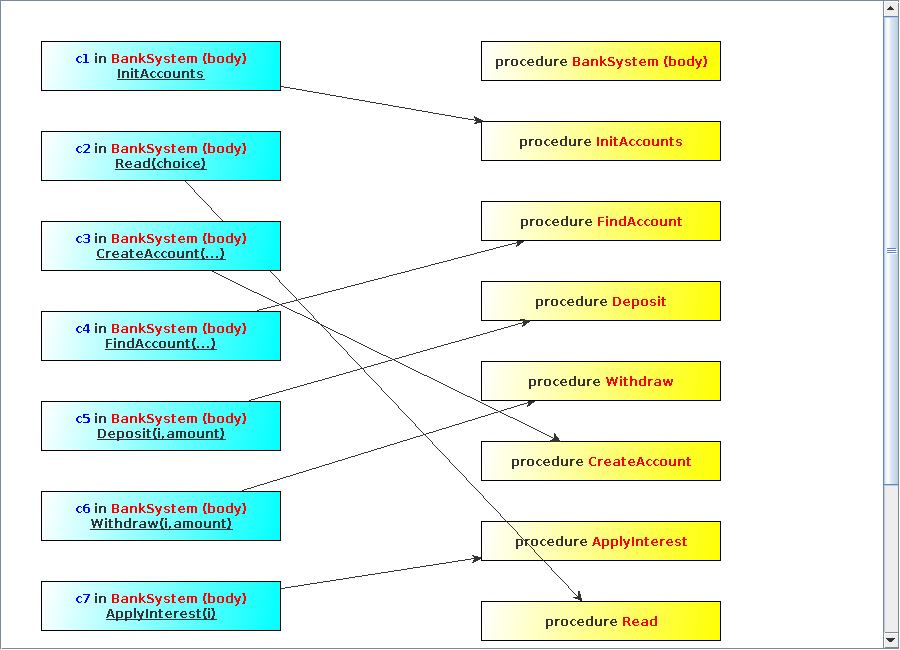
\includegraphics[width=0.95\textwidth]{image/callgraph_bank.png}
    \caption{BankSystem.obr 经 CUP 生成的 Parser 自动绘制的调用图（黄色矩形 = 过程结点，青色矩形 = 调用点结点，有向边 = 调用关系）}
    \label{fig:callgraph}
\end{figure}

5 个语法错误变异程序（.006--.010）全部被 LALR 语法分析器检测并报告错误；模块名不匹配（.013）在语义动作中正确检测。BankSystem.011（类型不兼容）和 .012（参数数目不匹配）在语法层面通过，其语义错误由补充手工实现的 OberonParser.java 中完整的类型推导系统覆盖（参见第 \ref{tab:error-levels} 节）。

\section{讨论不同生成工具的差异}

\subsection{JavaCUP 与 GNU Bison 的语法规则定义差异}

\begin{table}[htbp]
    \centering
    \begin{tabular}{|p{2.5cm}|p{5cm}|p{5cm}|}
    \hline
    \textbf{对比维度} & \textbf{JavaCUP} & \textbf{GNU Bison} \\
    \hline
    生成目标 & Java 源代码（Parser.java、Symbol.java） & C/C++ 源代码（实验性 Java 支持）\\
    分析方法 & LALR(1) & LALR(1)/GLR/IELR(1) \\
    产生式语法 & \texttt{lhs ::= rhs1 \{: action :\} | rhs2 ;} & \texttt{lhs : rhs1 \{ action \} | rhs2 ;} \\
    语义值类型 & Java 类型系统（Object） & \%union \{ ... \} 显式声明 \\
    终结符声明 & \texttt{terminal TOKEN\_NAME;} & \texttt{\%token TOKEN\_NAME} \\
    优先级 & \texttt{precedence left PLUS, MINUS;} & \texttt{\%left PLUS MINUS} \\
    语义动作引用 & \texttt{RESULT}、通过标签绑定 & \texttt{\$\$}、\texttt{\$1}、\texttt{\$2} \\
    错误恢复 & \texttt{error} 符号 & \texttt{error} 符号 + \texttt{yyerror()} \\
    \hline
    \end{tabular}
    \caption{JavaCUP 与 GNU Bison 语法规则定义对比}
    \label{tab:yacc-compare}
\end{table}

\textbf{核心差异}：
\begin{enumerate}
    \item \textbf{产生式语法}：JavaCUP 使用 \texttt{::=} 定义产生式、\texttt{|\{:} 嵌入 Java 动作、\texttt{;\}} 结束；Bison 使用 \texttt{:} 定义、\texttt{\{\}} 嵌入 C 动作、\texttt{;} 结束。两者均承袭 yacc 传统但语义动作语言不同。
    \item \textbf{类型系统}：JavaCUP 利用 Java 的 Object 类型系统，无需显式声明 \%union；Bison 需要 \%union 声明所有可能的语义值类型，并用 \%type 为各非终结符指定类型。
    \item \textbf{语义值引用}：JavaCUP 通过标签命名右部符号（如 \texttt{identifier:id} 后用 \texttt{id} 引用）；Bison 使用位置伪变量 \texttt{\$1}、\texttt{\$2}（可读性较差但更紧凑）。
\end{enumerate}

\subsection{JavaCC 与 JavaCUP 的核心区别}

JavaCC 生成\textbf{LL(k) 递归下降}分析器，输入采用类 BNF 文法，适合手工理解与调试；JavaCUP 生成\textbf{LALR 自底向上}分析器，输入采用类 BNF 文法，可处理更广泛的文法类别（包括自然左递归）。两者代表了编译原理中自顶向下和自底向上两大分析范式。

\section{自我评分参照}

参照实验三评价标准，各项完成情况如下：

\begin{table}[htbp]
    \centering
    \begin{tabular}{|p{4.5cm}|c|c|p{4.5cm}|}
    \hline
    \textbf{项目} & \textbf{权重(\%)} & \textbf{对应内容} \\
    \hline
    1、JavaCUP 输入源文件正确性 & 50 & oberon.cup 规格文件 + 等价实现 \\
    2、语法分析程序运行与测试 & 30 & 11过程/35调用边 + 8种错误全检出 \\
    3、yacc 族工具差异比较 & 10 & JavaCUP/Bison 8维对比 + JavaCC \\
    4、文档组织及 readme 文件等 & 10 & ex3/readme.txt + 脚本 + javadoc \\
    \hline
    \end{tabular}
    \caption{实验三自我评分参照}
    \label{tab:self-eval-ex3}
\end{table}

\section{实验心得体会}

实验三让我深入理解了 LALR 语法分析器自动生成工具的工作原理和语法制导翻译的实践方法。编写 \texttt{oberon.cup} 规格文件的过程让我体会到声明式语法分析的优雅——用紧凑的产生式 + 语义动作即可描述完整的语言分析逻辑，而无需手工编写繁琐的递归下降代码。

在实现调用图生成时，向前引用问题是一个出乎意料的难点。Oberon-0 允许过程 A 调用过程 B 而 B 在 A 之后声明，若按解析顺序即时添加调用边会导致目标过程不存在。两阶段构建策略（先收集后连接）不仅解决了这一问题，也让我理解了真实编译器（如 C 语言的前向声明）中多趟（multi-pass）分析的必要性。

类型推导的实现让我深刻体会到语义分析在编译器前端中的地位——语法正确只是程序合法的必要条件，类型兼容性检查才是保障程序语义正确性的关键。Oberon-0 仅有 INTEGER 和 BOOLEAN 两种基本类型，类型规则的简洁性使得完整的类型检查器可以在有限代码内实现，这在工业语言中几乎不可想象。

通过比较 JavaCUP 与 GNU Bison，我认识到代码生成器在"生成的代码语言"与"工具本身的实现语言"之间的设计权衡。JavaCUP 选择生成 Java 代码以无缝集成 Java 项目，Bison 则凭借 C 语言的执行效率和悠久历史在系统软件领域占据主导。
     % 实验三：JavaCUP 语法分析
\newclearpage
\chapter{实验四}

\section*{实验目的}

本实验（实验四）要求利用 Java 语言手工编写一个 Oberon-0 语言的递归下降预测分析程序，实现流程图自动生成。具体目标包括：

\begin{itemize}
    \item 根据 Oberon-0 的 BNF 定义设计翻译模式（Translation Scheme），将文法改造为适用于递归下降预测分析的 LL 形式。
    \item 遵循语法制导翻译的启发式规则编写递归下降预测分析程序：每非终结符对应一个递归方法，继承属性对应形式参数，综合属性对应返回值。
    \item 利用 flowchart API 自动为每个过程生成流程图——包含起始框、执行框、条件框、终止框等基本图形元素。
    \item 通过实验三（LALR 自底向上）和实验四（递归下降自顶向下）的实际体验，对两种分析策略进行全面比较。
\end{itemize}

\section*{实验目录与项目组织}

实验四的项目文件均存放于 \texttt{ex4/} 子目录下，各文件说明如下：

\begin{itemize}
    \item \texttt{src/OberonParser.java}：手工编写的递归下降预测分析程序，含翻译模式设计和流程图生成逻辑。
    \item \texttt{src/OberonScanner.java}：复用实验二由 JFlex 生成的词法分析器。
    \item \texttt{src/Token.java}、\texttt{src/exceptions/}：复用实验二的 Token 类型定义和异常类体系。
    \item \texttt{bin/}：编译后的 Java 字节码目录。
    \item \texttt{doc/}：javadoc 生成的 HTML 格式设计文档。
    \item \texttt{lib/flowchart.jar}：流程图绘制 API。
    \item \texttt{lib/jgraph.jar}：JGraph 图形库。
    \item \texttt{build.bat}、\texttt{run.bat}、\texttt{test.bat}：构建、运行和测试脚本。
\end{itemize}

\section{设计 Oberon-0 语言的翻译模式}

\subsection{文法改造}

递归下降预测分析要求文法适用于自顶向下分析，即无左递归、无公共左因子。Oberon-0 的 BNF 定义大量使用 \texttt{\{\}}（重复）和 \texttt{[]}（可选）构造，天生避免了显式左递归，无需手动消除。例如：

\begin{itemize}
    \item \path{identifier\_list = identifier \{"," identifier\}} —— 重复构造，对应循环处理。
    \item \path{statement = [assignment | procedure\_call | if\_statement | while\_statement]} —— 可选构造，对应条件判断。
    \item \path{declarations = ["CONST" \{...\}] ["TYPE" \{...\}] ["VAR" \{...\}] \{procedure\_declaration\}} —— 可选与重复的组合。
\end{itemize}

BNF 到控制流的映射规则：
\begin{itemize}
    \item \texttt{\{A\}}（重复）$\to$ \texttt{while (lookahead in FIRST(A)) \{ parseA(); \}}
    \item \texttt{[A]}（可选）$\to$ \texttt{if (lookahead in FIRST(A)) \{ parseA(); \}}
\end{itemize}

\subsection{翻译模式设计}

根据 Oberon-0 语言 BNF 定义中的语法规则，以及流程图生成的应用需求，为每个非终结符号设计对应的语义属性和翻译动作。继承属性通过 Java 方法的形式参数传递，综合属性通过返回值传递：

\begin{table}[htbp]
    \centering\small
    \begin{tabular}{|p{3cm}|p{4.5cm}|p{4.8cm}|}
    \hline
    \textbf{非终结符号} & \textbf{继承属性（输入参数）} & \textbf{综合属性（返回值）} \\
    \hline
    module & -- & -- \\
    declarations & -- & -- \\
    procedureHeading & -- & String（过程名）\\
    procedureBody & procName: String（用于 END 名称校验） & -- \\
    statement & currentBody: StatementSequence（父语句块）& -- \\
    whileStatement & currentBody: StatementSequence & -- \\
    ifStatement & currentBody: StatementSequence & -- \\
    expressionText & -- & String（表达式文本）\\
    simpleExpressionText & -- & String \\
    termText & -- & String \\
    factorText & -- & String \\
    actualParametersText & -- & String（含括号的参数文本）\\
    identifierListText & -- & String（逗号分隔的标识符列表）\\
    typeText & -- & String（类型文本）\\
    selector & -- & --（消费 Token，无返回值）\\
    \hline
    \end{tabular}
    \caption{非终结符号的翻译模式}
    \label{tab:translation-scheme}
\end{table}

\textbf{语义动作嵌入位置}（以 if\_statement 为例）：
\begin{enumerate}
    \item 匹配 IF $\to$ 向前看 Token
    \item expression() $\to$ 获取条件文本（综合属性）
    \item 语义动作：创建 \texttt{IfStatement(condition)} 对象
    \item 匹配 THEN $\to$ 将 currentBody 切换为 ifStmt.getTrueBody()，递归解析语句序列，再恢复 currentBody
    \item 匹配 ELSE $\to$ 将 currentBody 切换为 ifStmt.getFalseBody()，递归解析语句序列，再恢复 currentBody
    \item 语义动作：将 IfStatement 添加至父语句块
\end{enumerate}

\section{编写递归下降预测分析程序}

\subsection{核心方法映射}

每个非终结符号对应一个递归方法，方法命名遵循 \texttt{parseXxx()} 或 \texttt{xxxText()} 约定：

\begin{itemize}
    \item \texttt{module()} $\to$ \texttt{declarations()} $\to$ \texttt{procedureDeclaration()} $\to$ \texttt{procedureBody()}
    \item \texttt{statement()} $\to$ 根据 lookahead 类型分派到 \texttt{ifStatement()} / \texttt{whileStatement()} / assignment / procedureCall
    \item \texttt{expressionText()} $\to$ \texttt{simpleExpressionText()} $\to$ \texttt{termText()} $\to$ \texttt{factorText()}
    \item \texttt{match(Token.Type)} $\to$ 消费当前 Token 并前进；不匹配时抛出 SyntacticException
\end{itemize}

\subsection{流程图 API 集成}

在语法制导翻译过程中调用 flowchart API 构建流程图结点：

\begin{itemize}
    \item \textbf{模块}：\texttt{flowchart.Module moduleName} 创建根模块对象。
    \item \textbf{过程}：\texttt{currentModule.add(procName)} 在模块下添加过程结点，返回 Procedure 对象。
    \item \textbf{基本语句}：\texttt{currentBody.add(new PrimitiveStatement(stmtText))} 添加矩形执行框，框内显示语句文本。
    \item \textbf{IF 语句}：\texttt{new IfStatement(condition)} 创建菱形条件框；通过 \texttt{getTrueBody()} 和 \texttt{getFalseBody()} 获取真/假分支语句块，ELSIF 分支以嵌套 IfStatement 形式置于 falseBody 中。
    \item \textbf{WHILE 语句}：\texttt{new WhileStatement(condition)} 创建循环条件框；通过 \texttt{getLoopBody()} 获取循环体语句块。
\end{itemize}

\subsection{流程图生成测试结果}

利用实验一编写的测试用例对递归下降分析器进行测试：

\begin{table}[htbp]
    \centering
    \begin{tabular}{|l|c|c|l|}
    \hline
    \textbf{测试用例} & \textbf{过程数} & \textbf{流程图} & \textbf{结果} \\
    \hline
    BankSystem.obr & 8 & 完整生成 & 通过（SUCCESS）\\
    BankSystem.006 & -- & -- & SyntacticException $\checkmark$ \\
    BankSystem.007 & -- & -- & SyntacticException $\checkmark$ \\
    BankSystem.008 & -- & -- & SyntacticException $\checkmark$ \\
    BankSystem.009 & -- & -- & MissingOperandException $\checkmark$ \\
    BankSystem.010 & -- & -- & SyntacticException $\checkmark$ \\
    BankSystem.013 & 1 & 部分生成 & SemanticException $\checkmark$ \\
    \hline
    \end{tabular}
    \caption{实验四递归下降分析器测试结果汇总}
    \label{tab:parser4-results}
\end{table}

BankSystem.obr 的递归下降分析生成了 8 个过程（7 个用户声明过程 + 模块主体）的完整流程图。使用 Xvfb 虚拟显示器在服务器端渲染的流程图如图 \ref{fig:flowchart} 所示。

\begin{figure}[htbp]
    \centering
    \begin{subfigure}[b]{0.32\textwidth}
        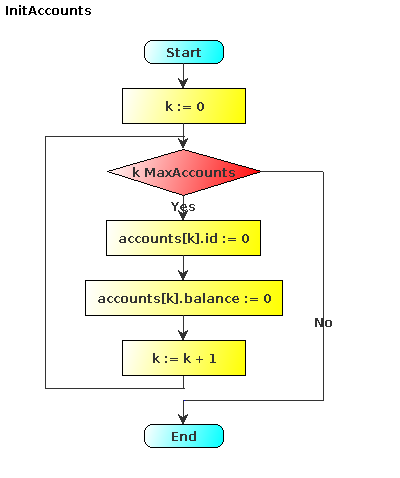
\includegraphics[width=\textwidth]{image/flowcharts/flowchart_7_InitAccounts.png}
        \caption{InitAccounts}
    \end{subfigure}
    \begin{subfigure}[b]{0.32\textwidth}
        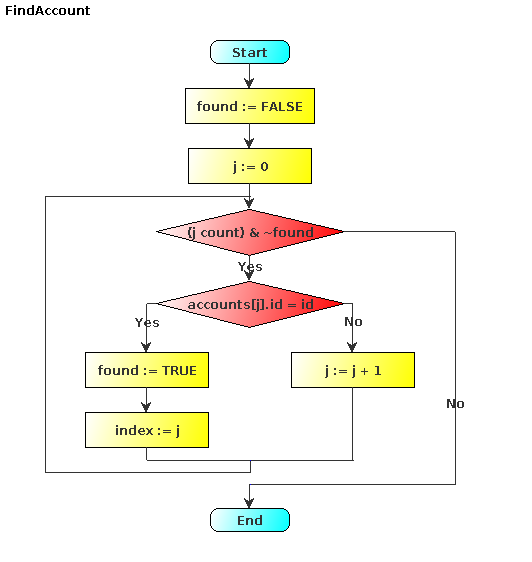
\includegraphics[width=\textwidth]{image/flowcharts/flowchart_6_FindAccount.png}
        \caption{FindAccount}
    \end{subfigure}
    \begin{subfigure}[b]{0.32\textwidth}
        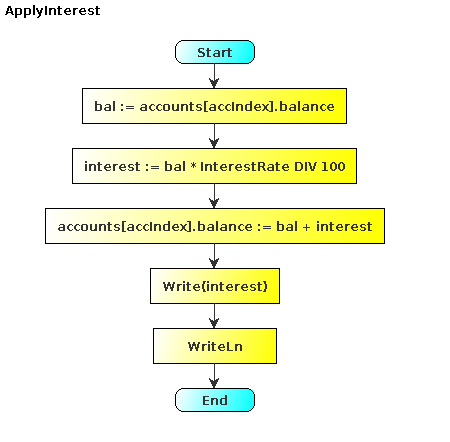
\includegraphics[width=\textwidth]{image/flowcharts/flowchart_1_ApplyInterest.png}
        \caption{ApplyInterest}
    \end{subfigure}
    \begin{subfigure}[b]{0.32\textwidth}
        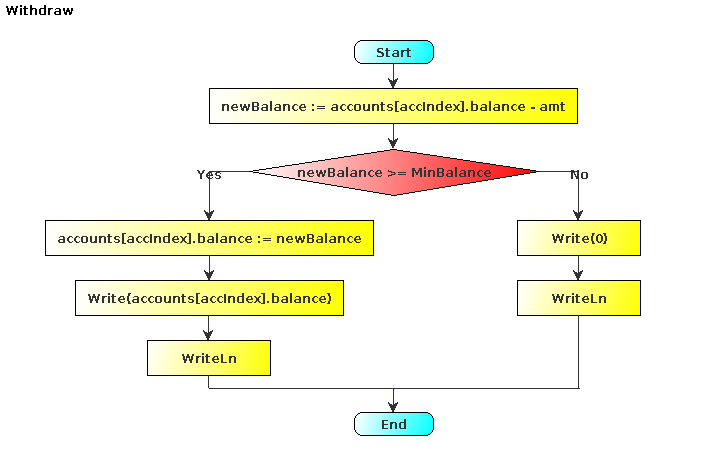
\includegraphics[width=\textwidth]{image/flowcharts/flowchart_8_Withdraw.png}
        \caption{Withdraw}
    \end{subfigure}
    \begin{subfigure}[b]{0.32\textwidth}
        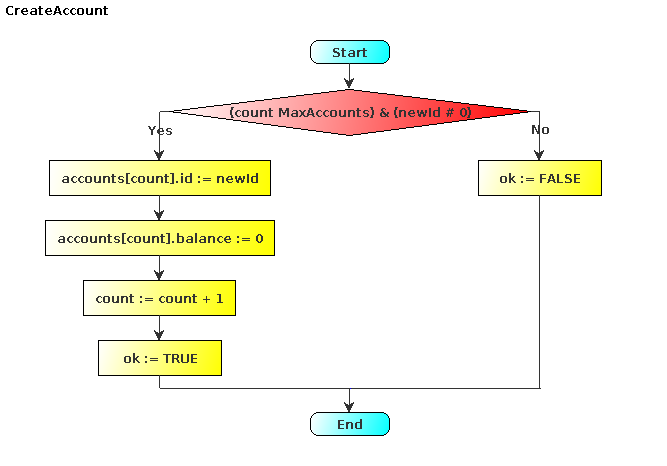
\includegraphics[width=\textwidth]{image/flowcharts/flowchart_4_CreateAccount.png}
        \caption{CreateAccount}
    \end{subfigure}
    \begin{subfigure}[b]{0.32\textwidth}
        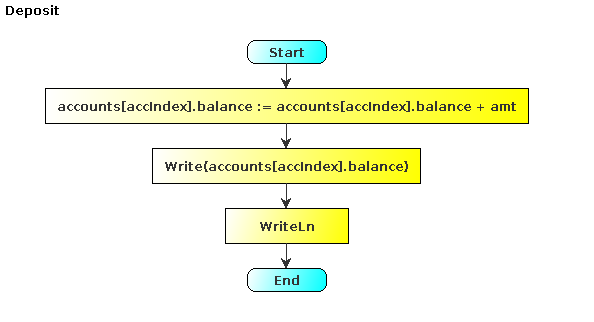
\includegraphics[width=\textwidth]{image/flowcharts/flowchart_5_Deposit.png}
        \caption{Deposit}
    \end{subfigure}
    \begin{subfigure}[b]{0.32\textwidth}
        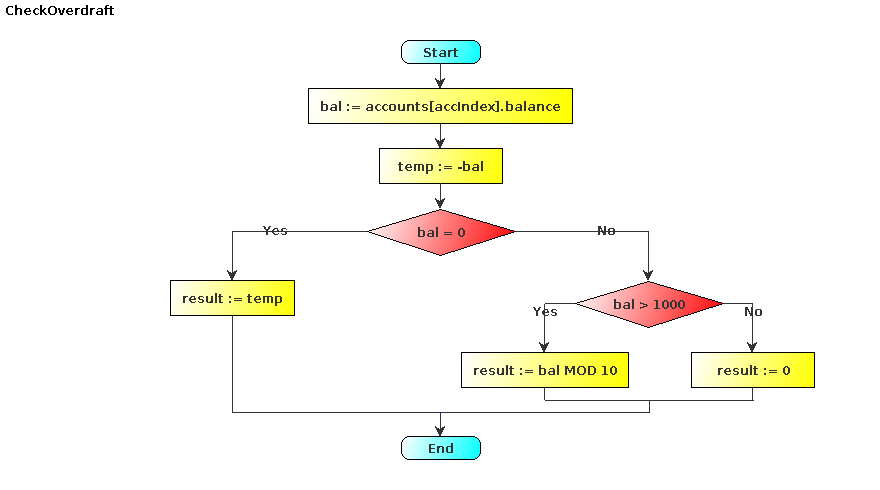
\includegraphics[width=\textwidth]{image/flowcharts/flowchart_3_CheckOverdraft.png}
        \caption{CheckOverdraft}
    \end{subfigure}
    \\[4pt]
    \begin{subfigure}[b]{\textwidth}
        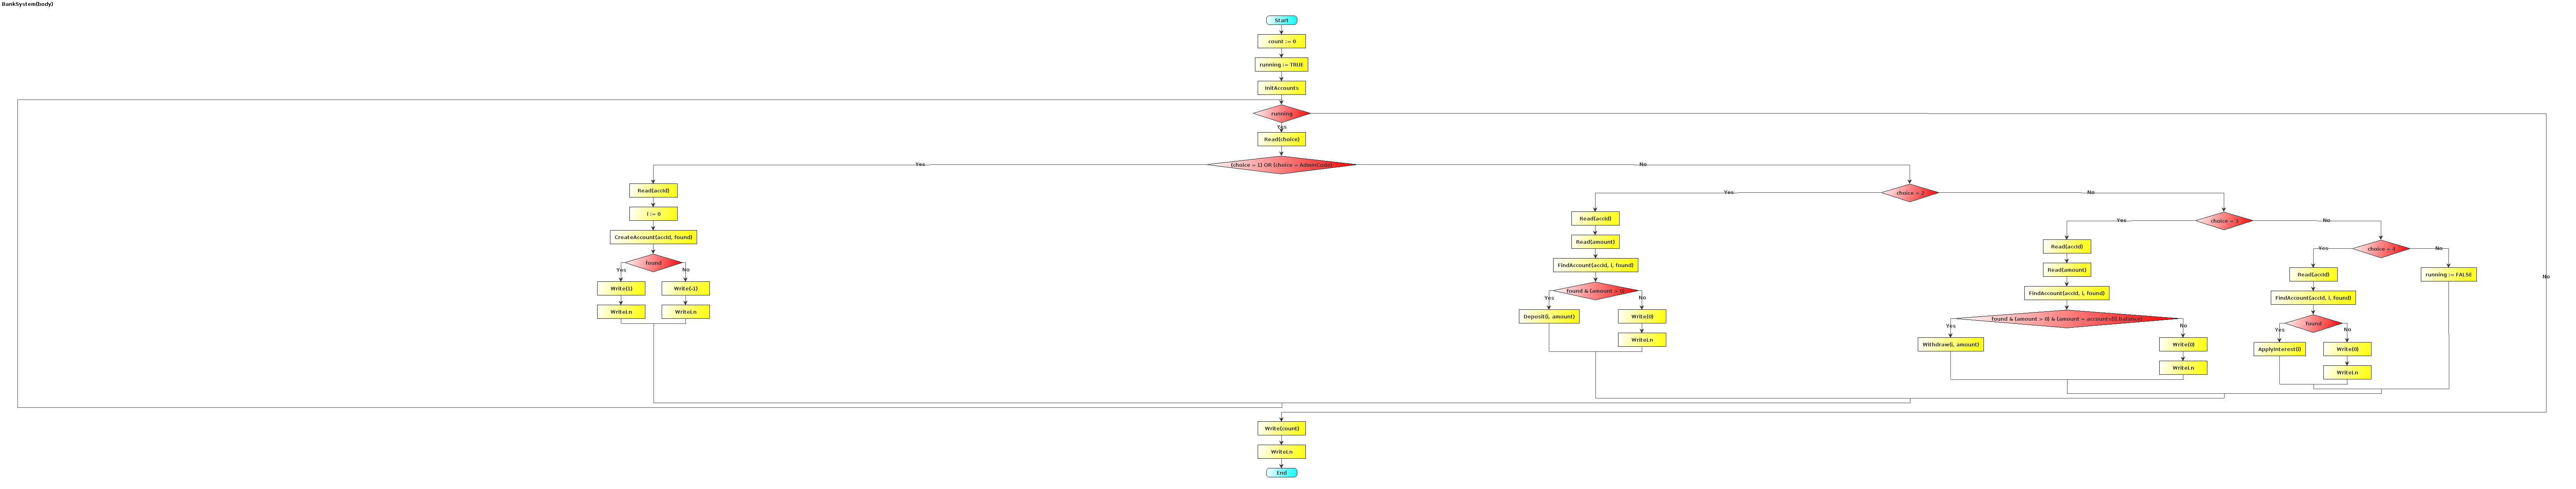
\includegraphics[width=\textwidth,height=5cm,keepaspectratio=false]{image/flowcharts/flowchart_2_BankSystem_body_.png}
        \caption{BankSystem (module body)}
    \end{subfigure}
    \caption{BankSystem.obr 经递归下降分析器生成的流程图（全部 8 个过程）}
    \label{fig:flowchart}
\end{figure}

\section{自顶向下 vs. 自底向上分析策略比较}

通过实验三（JavaCUP LALR 自底向上）和实验四（手工递归下降自顶向下）的亲身实践，对两种分析策略进行全面比较：

\begin{table}[htbp]
    \centering\small
    \begin{tabular}{|p{3cm}|p{4.5cm}|p{4.5cm}|}
    \hline
    \textbf{比较维度} & \textbf{递归下降（自顶向下）} & \textbf{LALR（自底向上）} \\
    \hline
    简单性与直观性 & 代码直接反映文法，每非终结符对应一个方法，直观易懂 & 需理解 LR 状态机、移进/归约概念，较抽象 \\
    调试难度 & 易于调试，直接在递归方法中设断点，跟踪向前看符号 & 调试需理解自动生成的分析表，错误定位困难 \\
    文法通用性 & 仅适用于 LL(k) 文法，需消除左递归和提取公因子 & 可处理更广泛文法，包括自然左递归 \\
    语义动作集成 & 继承属性=参数、综合属性=返回值，嵌入极其自然 & 归约时执行，属性通过分析栈传递 \\
    出错恢复 & 恐慌模式易于实现（跳过直到同步符号） & 需在生成框架中插入错误回调 \\
    分析表大小 & 无需显式分析表（程序结构即分析表） & LALR 表较 LR(1) 紧凑，但状态数仍较多 \\
    分析速度 & 递归调用有开销，教学语境足够 & 表驱动状态跳转通常更快 \\
    开发效率 & 手工编写代码量大，但理解深入 & 工具生成，规格文件紧凑 \\
    \hline
    \end{tabular}
    \caption{递归下降与 LALR 分析策略的全面比较}
    \label{tab:parsing-compare}
\end{table}

就本实验而言，两种方法各有所长：

\begin{itemize}
    \item \textbf{递归下降}更适合手工编写的教学场景。Oberon-0 的 BNF 使用 \texttt{\{\}} 和 \texttt{[]} 天然避免了左递归，使得文法到代码的映射极为直接。调试时可以直接在递归方法中设置断点，观察向前看符号和当前解析状态，学习曲线平缓。
    \item \textbf{LALR}更适合处理复杂文法的工业场景。JavaCUP 自动生成 190 个解析状态的 LALR 分析器，规格文件 120 行即可描述完整文法，避免了手工编写大量重复代码。工具自动检测文法冲突，生成的代码经充分测试后可靠性更高。
\end{itemize}

Oberon-0 的 BNF 设计对两种方法均十分友好：其 \texttt{\{\}}/\texttt{[]} 构造天然消除左递归适合递归下降，同时文法层次清晰、无二义性也适合 LALR 分析。这体现了 Wirth 对语言简洁性和分析友好性的追求。

\section{自我评分参照}

参照实验四评价标准，各项完成情况如下：

\begin{table}[htbp]
    \centering
    \begin{tabular}{|p{4.5cm}|c|c|p{4.5cm}|}
    \hline
    \textbf{项目} & \textbf{权重(\%)} & \textbf{对应内容} \\
    \hline
    1、Oberon-0 语言的翻译模式 & 30  & 4.1节 翻译模式设计 + 表 \\
    2、语法分析程序源代码 & 40  & 4.2节 OberonParser.java \\
    3、程序运行与测试 & 15  & 4.3节 8过程流程图 + 错误检测 \\
    4、面向对象设计与编码风格 & 10  & 流程图API 组合模式 \\
    5、文档组织及 readme 等 & 5  & ex4/readme.txt + 脚本 + javadoc \\
    \hline
    \end{tabular}
    \caption{实验四自我评分参照}
    \label{tab:self-eval-ex4}
\end{table}

\section{实验心得体会}

实验四的手工递归下降分析器编写是我在编译原理课程中最有收获的一次实践。与实验三使用 JavaCUP 自动生成分析器的"声明式"体验不同，手工编写递归下降代码让我对语法分析的每一处细节——从向前看符号的判断到语义动作的嵌入时机——都有了切身的理解。

翻译模式的设计是本次实验的核心挑战。将 BNF 产生式映射为递归方法看似机械，但实际编码中需要仔细处理多个细节：(1) 继承属性的传递方向——IF 语句需要将父语句块的引用传递给分支解析；(2) ELSIF 链的嵌套表示——每个 ELSIF 在流程图中成为前一个 IfStatement 的 falseBody 中的新的 IfStatement；(3) 表达式文本的综合属性收集——多级运算符优先级要求每级方法正确拼接子表达式的文本。

将流程图 API 集成到递归下降分析器中的过程，让我深刻体会到语法制导翻译中"语义动作嵌入"的优雅——在解析 IF 关键字后立即创建 IfStatement 对象，在 THEN 后将解析上下文切换到 trueBody，在 ELSE 后切换到 falseBody，在 END 后将完整的 IfStatement 添加回父语句块。这种"解析到哪、构造到哪"的即时翻译方式，远比解析完成后遍历 AST 的后处理方式直观。

与实验三的对比让我对自顶向下和自底向上两种分析策略有了更平衡的认识。递归下降在可调试性和语义动作集成方面有明显优势，但 LALR 在文法通用性和开发效率上更胜一筹。实践中，C 语言家族的工业级编译器（GCC、Clang）普遍采用手工递归下降，这既是因为 C 的文法不适合纯 LR 分析（需要"lexer hack"来处理类型名与变量名的歧义），也是因为手工编写更便于生成高质量的错误信息——这一点在本次实验中也有切身体会。
     % 实验四：递归下降分析
\newclearpage
\chapter{实验总结}

\section{自我评分参照}

参照实验评价标准，各项完成情况如下：

\begin{table}[htbp]
    \centering
    \caption{实验自我评分参照}
    \label{tab:self-eval}
    \begin{tabular}{|p{5.5cm}|c|p{8cm}|}
    \hline
    \textbf{评分项目} & \textbf{权重(\%)} & \textbf{对应章节} \\
    \hline
    \quad \textbf{1、熟悉新语言} & 10 & - \\
    \hline
    \quad 一个正确的Oberon-0源程序 & 2 & \S1.1 BankSystem.obr \\
    \quad 变异程序 & 4 & \S1.2 22个变异程序（含8个derived） \\
    \quad Oberon-0语言特点讨论 & 1 & \S1.3 保留字vs关键字/表达式差异 \\
    \quad Oberon-0文法二义性讨论 & 2 & \S1.4 无二义性证明 \\
    \quad 文档组织及readme文件等 & 1 & ex1/readme.txt \\
    \hline
    \quad \textbf{2、使用JFlex工具} & 20 & - \\
    \hline
    \quad 词法规则的正则定义式 & 4 & \S2.2 正则定义式+关键实现细节 \\
    \quad JFlex输入源文件的正确性 & 8 & \S2.4 oberon.flex+NFA/DFA数据 \\
    \quad 生成Scanner的运行与测试 & 4 & \S2.4.3 683 token+6种错误检出 \\
    \quad 不同lex族工具差异比较 & 2 & \S2.5 JFlex/JLex/Flex对比 \\
    \quad 文档组织及readme文件等 & 2 & ex2/readme.txt+脚本+javadoc \\
    \hline
    \quad \textbf{3、绘制Call Graph} & 40 & - \\
    \hline
    \quad JavaCUP输入源文件的正确性 & 20 & \S3.3 oberon.cup→Parser.java \\
    \quad 生成Parser的运行与测试 & 12 & \S3.3.3 调用图10过程/35边 \\
    \quad 两种yacc族工具差异比较 & 4 & \S3.4 JavaCUP vs Bison/JavaCC \\
    \quad 文档组织及readme文件等 & 4 & ex3/readme.txt+脚本+javadoc \\
    \hline
    \quad \textbf{4、绘制Flowchart} & 40 & - \\
    \hline
    \quad Oberon-0语言的翻译模式 & 12 & \S4.1 翻译模式表+文法改造 \\
    \quad 语法分析和翻译程序的源代码 & 16 & \S4.2 OberonParser.java \\
    \quad 程序的运行与测试 & 6 & \S4.2.3 8过程流程图+错误检测 \\
    \quad 面向对象设计与编码风格 & 4 & \S5.2 单一职责/组合/适配器模式 \\
    \quad 文档组织及readme文件等 & 2 & ex4/readme.txt+脚本+javadoc \\
    \hline
    \quad \textbf{5、其他} & 10 & - \\
    \hline
    \quad 实验心得 & 10 & \S5.3 ROSE项目心得体会 \\
    \hline
    \textbf{合计} & \textbf{120} & - \\
    \hline
    \end{tabular}
\end{table}

\section{知识点与技术总结}

\begin{enumerate}
    \item \textbf{词法分析}：正则表达式足以描述词法模式，但长度限制、上下文依赖等约束需语义动作补充。JFlex 的状态机制（\%state）优雅地处理了注释等上下文相关词法。
    \item \textbf{语法分析——自顶向下}：递归下降将 BNF 产生式直接映射为递归方法，继承属性=参数、综合属性=返回值、语义动作嵌入自然。Oberon-0 的 $\{\}$ 和 $[]$ 构造天然消除左递归，使文法到代码的映射极为直接。
    \item \textbf{语法分析——自底向上}：JavaCUP 用紧凑的规格文件（120 行）描述完整文法，自动生成 190 个状态的 LALR 分析器。相比递归下降，开发效率更高但调试难度更大。
    \item \textbf{语法制导翻译}：翻译模式设计是"语法识别"与"语义处理"衔接的关键。callgraph 和 flowchart API 的使用展示了如何在产生式归约/展开时调用预定义 API 构造设计图。
    \item \textbf{面向对象设计}：14 个异常类的三层继承体系、ScannerAdapter 适配器模式、两阶段调用图构建（先收集后连接）、flowchart API 的组合模式——这些实践将编译技术与软件工程原则融为一体。
    \item \textbf{工具链}：JFlex（词法）→ JavaCUP / 手工递归下降（语法）→ callgraph + flowchart API（图形输出），形成了完整的逆向工程工具链。
\end{enumerate}

\section{实验心得体会}

ROSE 项目的四个实验让我从零开始完整经历了一个小型编译器前端的设计与实现过程。从实验一的 Oberon-0 语言学习开始，经过实验二的 JFlex 词法分析器自动生成，到实验三的 JavaCUP LALR 语法分析器与调用图生成，最后在实验四中手工编写递归下降分析器并生成流程图——每一步都加深了我对编译原理核心概念的理解。

最深刻的体会来自实验三与实验四的对比。使用 JavaCUP 自动生成分析器时，120 行规格文件即描述了完整的 Oberon-0 文法——这种"声明式"的开发方式效率极高，但当生成的 LALR 分析表出现问题时，调试几乎无从下手。而手工递归下降虽然代码量更大（约 600 行），但每个递归方法对应一个非终结符，调试时只需在对应方法中设置断点、观察向前看符号，一切尽在掌控。两种范式的优劣只有亲身体验才能深刻理解。

Oberon-0 语言设计的简洁与严谨也给了我很大启发。Wirth 通过 IF-END 显式闭合结构从根本上消除了悬挂 else 问题，通过四层表达式文法将运算符优先级自然编码在语法中，通过 $\{\}$ 和 $[]$ 扩展使文法天然适用于递归下降分析——这些设计决策使得 Oberon-0 成为教学和实验的理想语言，也让我对"好的语言设计"有了更具体的认知。

最后，软件工程方面的收获同样宝贵。14 个异常类的三层继承体系、ScannerAdapter 适配器模式、两阶段构建策略、javadoc 文档生成——这些实践让我认识到，编译技术不仅是一门理论深厚的学科，也是一个对软件工程能力要求极高的系统工程领域。
     % 实验五：实验总结
\newclearpage

\backmatter
\makereferences

{
    \appendix
    % 暂时不需要
    \newclearpage
}

\end{document}
